\chapter{Experimentálna časť}
\label{part:Aplikacia}

V tejto poslednej kapitole sa budeme venovať návrhu aplikácie, pomocou ktorej môžeme využívať decentralizované MPC s možnosťou paralelného riešenia na viacerých výpočtových zariadeniach. V rámci aplikácie bude možné pracovať s rôznymi lineárnymi aj nelineárnymi modelmi systému. Výstupom z aplikácie bude vypočítaný optimálny akčný zásah v danej perióde vzorkovania. Ďalej budeme využívať tento výstup pri simulácií riadenia na definovanom modeli systému. Alternatívou by bolo nahradenie simulácie reálnym systémom, ale bolo by nutné zaviesť úpravy. 

Najskôr si ukážeme architektúru aplikácie, na základe ktorej sme neskôr vybudovali logiku celej aplikácie. V ďalšej časti si vysvetlíme nastavenie servera, ako s ním budeme komunikovať a spôsob ukladania dát v aplikácii. Následne na to si ukážeme rozhranie, s ktorým sa stretne používateľ. A posledné dve časti tejto kapitoly budú venované spôsobu fungovania aplikácie, rozoberieme si postupnosť logických krokov a overíme si ich na simulácií. 
\section{Architektúra aplikácie}
Aplikáciu delíme na dve časti, prvá je serverová a bude naprogramovaná v jazyku Python pomocou knižnice Flusk. Druhú časť nazývame klientská a bude sa nachádzať vo webovom rozhraní.
\label{fig:ArchitekturaAPK}
\begin{figure}[H]	
	\centering
	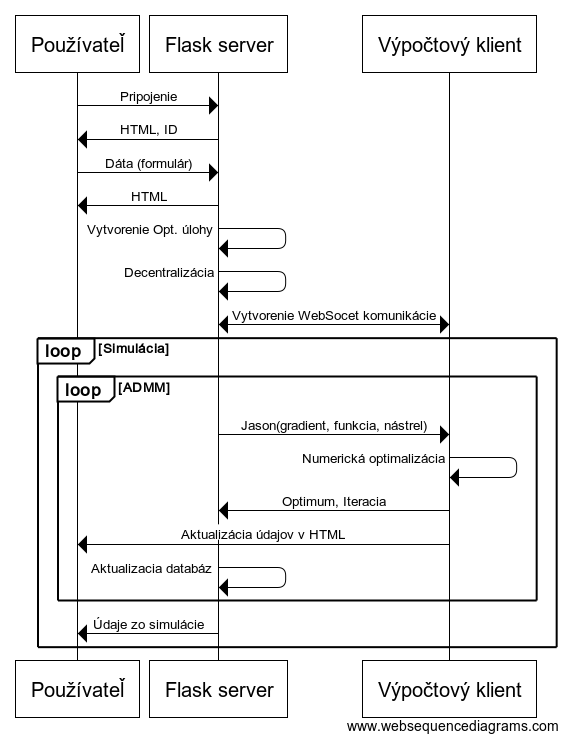
\includegraphics[width=13cm,height=18cm]{images/Aplikacia}
	\caption{Zjednodušený diagram aplikácie pre jedného klienta}
\end{figure}
\newpage
Na (Obr. 4.1) môžeme vidieť architektúru, ktorá slúžila ako základ pre našu aplikáciu. Klientska čast sa bude deliť na dve, prvá je používateľské rozhranie, v ňom bude klient môcť ovládať simuláciu a sledovať výsledky z optimalizácie. Druhá časť je takzvaný výpočtový klient, táto časť bude reprezentovať numerickú optimalizáciu, ktorá bude prebiehať na pozadí prehliadača v JavaScripte. 
\section{Server}
Ako sme už spomínali, pre vytvorenie servera použijeme knižnicu Flask. Táto knižnica obsahuje micro web framwork pre programovací jazyk Python, inak povedané, podporuje vývoj webovej aplikácie, konkrétne web server. Nazývaný je micro, lebo je navrhnutý tak, aby jeho jadro bolo čo najjednoduchšie, ale podporuje rozšíriteľnosť pomocou už existujúcich knižníc. To je zároveň aj jeho najväčšia výhoda, nie je dopredu určené, aký druh databáz musíme používať, alebo v akej forme budeme odosielať a prijímať dáta, vo všetkom má developer voľnosť.
\subsection{Nastavenie servera}
Nastavenie servera je veľmi jednoduché, stačí importovať knižnicu Flask,
\begin{lstlisting}[language=Python]
from flask import Flask
\end{lstlisting}\noindent
vytvoríme si premennú, ktorá bude reprezentovať náš server.
\begin{lstlisting}[language=Python]
app = Flask(__name__)
\end{lstlisting}\noindent
Ďalej je potrebné určiť, čo sa stane, keď sa klient pripojí na server. V nasledujúcom príklade odkážeme klienta na html stránku
\begin{lstlisting}[language=Python]
@app.route('/')
	return render_template('index.html')
\end{lstlisting}\noindent
a nakoniec si zadefinujeme, na akom porte bude náš server fungovať.
\begin{lstlisting}[language=Python]
if __name__ == '__main__':
	app.run(host='localhost', port=5000)
\end{lstlisting}
Takto nastavený server nájdeme na adrese http://localhost:5000/ rovnako ako náš, ktorý budeme poožívať v tomto projekte\cite{bib4}.

\subsection{Práca s databázou}
Vďaka voľnosti, ktorú nám poskytuje Flask, sme si mohli vybrať zo širokej škály knižníc pre prácu s dátami. V dnešnej dobe sú databázy najpoužívanejšou a veľmi efektívnou formou, ako ukladať, aktualizovať a spravovať údaje. Takto uložené dáta sú v tabuľkovej podobe, kde každý stĺpec má preddefinovaný formát a veľkosť a každý riadok stĺpca má priradený jedinečný index, ktorý uľahčuje SQL (Structured Query Language) prehľadávanie v databáze.

My sme v tejto práci využili knižnicu SQLAlchemy, konkrétne jej upravenú verziu FlaskSQLAlchemy. Umožňuje plné využívanie SQL pre prácu s databázami v našom Flask serveri, a to pomocou takzvaného ORM (Object Relational Mapper), čo je programovacia technika pre konvertovanie dát medzi nekompatibilnými systémami (programovacími jazykmi), čo je v našom prípade Python a SQL. 

Pomocou tejto knižnice sme si vytvorili štyri databázy, ktoré budeme používať v našej aplikácii. 
\label{DB:Klient}
\begin{enumerate}
\item{ Databáza klientov - v tejto databáze budeme mať uložených všetkých klientov, ktorý pracujú alebo pracovali na optimalizácii, štruktúra databázy je nasledovná:
\begin{lstlisting}[language=Python]
class Clients(db.Model):
__bind_key__ = 'Clients'
ID = db.Column(db.Integer, primary_key=True)
MPC_optimization_id = db.Column(db.Integer, index=True)
Date_created = db.Column(db.DateTime,\
                      default=datetime.utcnow)
Status = db.Column(db.Integer(2), index=True) 
\end{lstlisting}
}
\label{DB:OPT}
\item{ Databáza optimalizačných úloh - táto databáza bude obsahovať všetky optimalizačné problémy (MPC), ktoré si vytvoríme zo zadefinovaných informácií od klienta. Budeme ju ďalej používať ako základ pre decentralizovanú optimalizáciu. Hlavnou vlastnosťou tejto databázy bude, že sa naplní iba raz v rámci jedného MPC a tieto údaje budú nemenné počas chodu aplikácie. Obsahuje nasledovné informácie:
\begin{lstlisting}[language=Python]
class MPC_optimization(db.Model):
__bind_key__ = 'MPC_optimization'
ID = db.Column(db.Integer, primary_key=True)
General_Model = db.Column(db.String(5000), index=True)
General_Function = db.Column(db.String(10000), index=True)
Variable = db.Column(db.String(64), index=True)
Reference = db.Column(db.String(64), index=True)
Nmin = db.Column(db.String(64), index=True)
Nmax = db.Column(db.String(64), index=True)
Client_id = db.Column(db.Integer, index=True)
Status = db.Column(db.Integer(2), index=True)
\end{lstlisting}
}
\label{DB:WORKER}
\item{ Databáza distribuovaných optimalizačných úloh - táto databáza bude niesť informácie o distribuovanej optimalizačnej úlohe pre jednotlivých klientov. Na rozdiel od predošlej databázy, táto sa môže meniť počas chodu aplikácie, ale len vtedy, ak sa pripojí alebo odpojí klient z aplikácie. Databáza bude mať zadefinovanú nasledovnú podobu:
\begin{lstlisting}[language=Python]
class MPC_Worker(db.Model):
__bind_key__= 'MPC_Worker'
ID = db.Column(db.Integer, primary_key=True)
Optimization_Variables = db.Column(db.String(64), index=True)
Function = db.Column(db.String(5000), index=True)
Gradient = db.Column(db.String(10000), index=True)
Client_id = db.Column(db.Integer, index=True)
Status = db.Column(db.Integer(2), index=True)
\end{lstlisting}
}
\label{DB:WORKER_DATA}
\item{ Databáza výsledkov po optimalizácii - posledná databáza, s ktorou budeme pracovať v rámci tejto aplikácie. Na rozdiel od predošlých databáz, táto sa vytvorí pre každú optimalizovanú premennú a bude sa aktualizovať po každej optimalizácii. Štruktúra databázy je nasledovná:
\begin{lstlisting}[language=Python]
class MPC_Worker_data(db.Model):
__bind_key__= 'MPC_Worker_data'
ID = db.Column(db.Integer, primary_key=True)
Variable = db.Column(db.String(64), index=True)
Optimal_value = db.Column(db.String(20), index=True)
Iteration = db.Column(db.Integer(20), index=True)
Client_id = db.Column(db.Integer, index=True)
Status = db.Column(db.Integer(2), index=True)
\end{lstlisting}
}
\end{enumerate}

\subsection{Komunikácia}
Komunikácia medzi serverom a klientom bude prebiehať dvoma rôznymi spôsobmi. Pre jednorázové akcie, ako je odoslanie formulára alebo pripojenie či odpojenie zo servera, využijeme HTTP requesty, konkrétne metódy POST a GET. Pre častú komunikáciu ako bude odosielanie dát na optimalizáciu alebo zmena referencie v simulácii je omnoho lepšou možnosťou otvoriť komunikačný kanál medzi serverom a klientom. Tento kanál bude sprostredkovávaný pomocou WebSocket protokolu a zjednoduší komunikáciu. Server tak bude môcť rovno odosielať dáta klientovi, bez toho aby o ne musel najskôr požiadať. 

\subsubsection{HTTP}
HTTP je skratka z angličtiny (Hypertext Transfer Protocol) a predstavuje protokol, ktorý bol určený na výmenu hypertextových dokumentov medzi serverom a prehliadačom (klientom). Funguje na nasledovnom princípe, klient zašle požiadavku (request) a čaká na odpoveď zo strany servera, ktorý odpovedá zaslaním HTML súboru alebo iného obsahu, môže vykonať nejakú funkciu či odpovedať správou späť klientovi. \cite{bib5}

HTTP poskytuje viacero request metód, ktoré hovoria o tom, akú odpoveď očakáva klient zo strany servera. My budeme využívať dve najpoužívanejšie metódy.
\begin{enumerate}
\item { Metóda GET, zjednodušene povedané, slúži na vyžiadanie si dát zo špecifického zdroja. Táto požiadavka ostáva v histórii prehliadača a nemala by sa využívať pri práci s citlivými údajmi. V našej aplikácií ju budeme využívať pre presmerovanie klienta medzi HTML súbormi.  
}
\item { Metóda POST, sa využíva najmä pre odoslanie, vytváranie alebo aktualizovanie dát pre server. Táto požiadavka neostáva v histórii. My ju budeme využívať pre potvrdenie a odoslanie formulárov z webovej stránky na server.  
}
\end{enumerate}

\subsubsection{WebSockets}
WebSockets je iná forma prijímania a odosielanie dát medzi serverom a prehliadačom ako tomu bolo pri HTTP. Poskytuje komunikáciu v oboch smeroch (klient-server) cez jediné TCP (Transmission Control Protocol) pripojenie. Pomocou WebSocekt aplikácie vieme vytvoriť obojstrannú komunikáciu, kde klient môže cez prehliadač poslať správy (dáta) na server a tiež môže dostať odpoveď od servera na základe nejakých udalostí bez toho, aby o ne musel požiadať. \cite{bib6}

Na rozdiel od HTTP, na vytvorenie takejto komunikácie budeme potrebovať dve knižnice, jednu pre Flask server a druhú pre klienta (JavaScript). Na strane servera budeme využívať flask-SocetIO, táto knižnica nám zmení nastavenia servera (konkrétne definovanie portu) a to tak, že nám obalí pôvodný server. Zmena bude nasledovná.
\begin{lstlisting}[language=Python]
from flask_socketio import SocketIO
socketio = SocketIO(app)
if __name__ == '__main__':
	socketio.run(app, host='localhost', port=5000)
\end{lstlisting}
Pre JavaScript použijeme knižnicu Socet.IO, ktorú si pridáme pomocou webového linku. Je nutné sa pripojiť na adresu, kde bude komunikácia prebiehať, v našom prípade je to adresa servera \cite{bib3}.
\begin{lstlisting}[language=Java]
var socket = io.connect('http://localhost:5000/');
\end{lstlisting}

\section{Klientská časť}
Na strane klienta budeme mať jednoduché rozhranie, kde bude klient navádzaný pomocou tlačidiel a formulára na zadefinovanie MPC. Akonáhle sa odošlú údaje na server, klient bude presmerovaný na HTML stránku, kde už bude mať k dispozícií všetky informácie o optimalizácii a simulácii. Aby bola klientska časť zovšeobecnená, budeme vo webovom rozhraní používať iba anglický jazyk. V nasledujúcich dvoch častiach bude ukázané, s akým rozhraním sa klient stretne a okrajovo bude naznačené, čo sa bude vykonávať v JavaScripte, teda na pozadí stránky. V nasledujúcej podkapitole (4.3) si tieto veci viac priblížime. 
\subsection{Formulár}
\label{subse:Formular}
V tejto aplikácii budeme využívať iba jeden formulár. Ten sme si rozdelili na dve časti. V prvej sa zadefinuje model riadeného systému a všetky vstupné, výstupné a stavové premenné. Druhá čast slúži na definovanie optimalizačného problému (parametre prediktívneho regulátora). Všetky polia sa vypĺňajú pomocou maticového zápisu, rovnako ako v programovacom jazyku Matlab. Formulár sa po vyplnení odošle pomocou HTTP metódy POST na server, kde sa spracujú všetky informácie. 
\begin{enumerate}
\item {Nastavenie riadeného systému- v tomto formulári môžeme zadefinovať diskrétny model systému, buď ako stavový opis (lineárny model) alebo pomocou diferenciálnych rovníc (lineárny/nelineárny model).
\begin{figure}[H]	
	\centering
	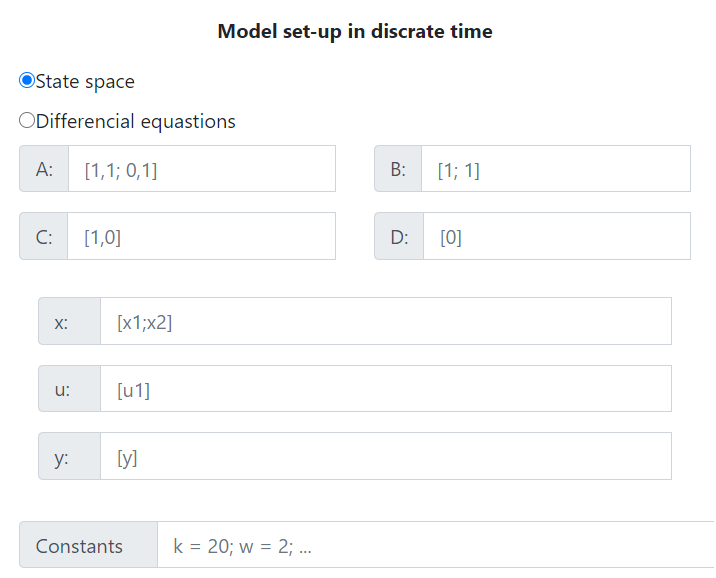
\includegraphics[width=11cm,height=8cm]{images/Model_setup}
	\caption{Formulár pre definovanie systému}
\end{figure}
V ľavom hornom rohu (Obr. 4.1) si môžeme vybrať z týchto dvoch možností a na základe výberu sa nám upravia vstupné polia. Na obrázku vyššie máme znázornený stavový opis systému, kde si zadefinujeme matice A a B. Ako sme už spomínali, v tomto projekte budeme uvažovať iba stavové riadenie, takže rovnica výstupu $y_{k} = Cx_{k} + Du_{k}$ nás nebude zaujímať, polia sú vytvorené pre prípadné zmeny v budúcnosti. V poliach x a u, zadefinujeme vstupné (u) a stavové (x) veličiny, môžu to byť ľubovolné názvy, ale pri použití diferenciálnych rovníc sa musia zhodovať s tým v rovniciach. Posledné pole pre konštanty slúži na definovanie konštánt, ktoré sa použili v poliach vyššie. Teda je možné predísť písaniu čísel do rovníc a môžeme ich nahradiť premennými. 
}
\item {Definovanie parametrov MPC.
\begin{figure}[H]	
	\centering
	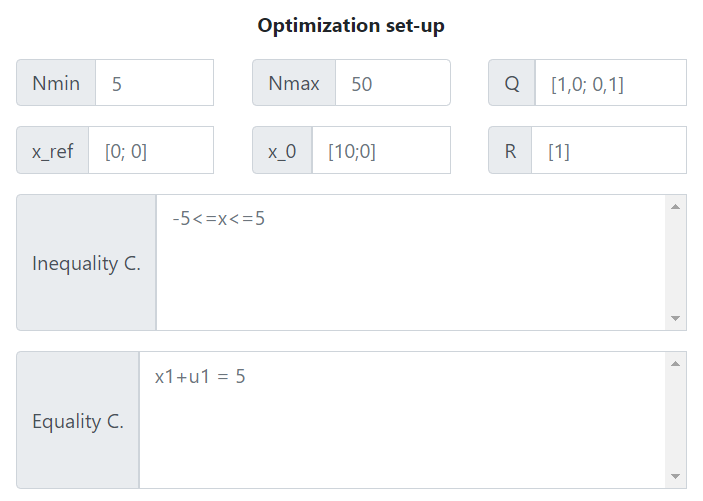
\includegraphics[width=11cm,height=8cm]{images/MPC_setup}
	\caption{Formulár pre definovanie MPC}
\end{figure}
Ako môžeme vidieť na (Obr. 4.2) máme celkovo osem polí pre definovanie predikatívneho regulátora, z toho dve nebudeme v tomto projekte používať a to $Nmax$, čo predstavuje maximálny predikčný horizont a rovnostné ohraničenia (Equality C.). Prvé pole $Nmin$ definuje minimálny predikčný horizont, $Q$ a $R$ sú váhové matice používané v MPC. Ďalej máme pole určené pre neostré nerovnostné ohraničenia (Inequality C.) a dve polia pre definovanie počiatočnej hodnoty stavov ($x_{0}$) a referencie, kam sa majú jednotlivé stavy dostať ($x_{ref}$).
}
\end{enumerate}
Súčasťou tohoto formulára je tiež validácia, ktorá sa spustí vždy pri odosielaní formulára. Prebieha v JavaScripte na strane klienta. Kontroluje, či sú zadefinované všetky potrebné polia a zároveň kontroluje, či majú všetky správne rozmery. Ak formulár neprejde validáciou, nebude odoslaný ďalej na server, a vyskočí okno pri danom poli s popisom chyby.
\subsection{Optimalizácia a simulácia}
\label{subse:OPTaSIM}
Akonáhle sa odošlú údaje z formulára časť \hyperref[subse:Formular]{(4.3.1)} na server, klient je presmerovaný na novú HTML stránku. Na tejto stránke bude v pozadí prebiehať Newtonova numerická optimalizácia  \hyperref[opt:Newton]{(2.5.2)}, táto optimalizácia bude naprogramovaná v jazyku JavaScript. Jej úlohou bude nájsť optimálne riešenie pre decentralizovaný optimalizačný problém. Výsledky z tejto optimalizácie budú zobrazené na stránke v nasledujúcom formáte. 
\label{fig:Tabulka}
\begin{figure}[H]	
	\centering
	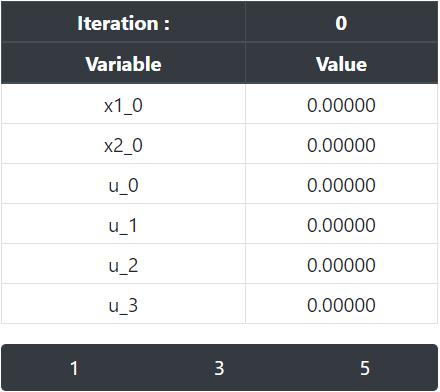
\includegraphics[width=6cm,height=6.5cm]{images/tabulka}
	\caption{Tabuľka výsledkov}
\end{figure}
Na (Obr. 4.3) môžeme vidieť príklad dynamickej tabuľky. Táto tabuľka zobrazuje všetky optimalizované premenné a ich hodnoty z jednotlivých optimalizácií. V tabuľke tiež môžeme nájsť, koľko iterácií trvalo numerickej optimalizácii, kým skonvergovala do optima. Po ukončení simulácie si môžeme pozrieť jednotlivé výsledky zo všetkých optimalizácií, ktoré klient vykonal a to pomocou tlačidiel nachádzajúcich sa pod tabuľkou.

Súčasťou tejto stránky je tiež zobrazenie simulácie riadeného systému. Táto simulácia prebieha na serveri, bude možné ju ovládať, a to pomocou zmeny referencie a zastavovacieho tlačidla.
\begin{figure}[H]	
	\centering
	
\includegraphics[width=9cm,height=1cm]{images/ovladanie_simulacie}
	\caption{Panel pre ovládanie simulácie}
\end{figure}
Na (Obr. 4.4) máme zobrazený panel, pomocou ktorého môžeme ovládať simuláciu zo strany klienta. Máme k dispozícii možnosť zastaviť prebiehajúcu simuláciu, alebo zmeniť žiadanú hodnotu pre jednotlivé stavy. Rovnako, ako v predchádzajúcej časti, aj tu sa zvalidujú údaje pred odoslaním. Ak prejdú validáciou, sú odoslané na server, kde sú spracované. Server odošle naspäť správu, či všetko prebehlo v poriadku.

Pre sledovanie simulácie budeme mať k dispozícii dva dynamické grafy, ktoré budú zobrazovať údaje v reálnom čase, a to pomocou JavaScript knižnice Chart.js. Táto knižnica je voľne dostupná na internete, bude nám poskytovať možnosť vytvorenia interaktívnych grafov a veľkú voľnosť, vďaka ktorej môžeme premeniť statické grafy na dynamické. Nad grafom bude zobrazená legenda s príslušnými veličinami, a tiež bude fungovať ako panel ovládania, pomocou ktorého môžeme pridávať a odoberať veličiny z grafu. 
\begin{figure}[H]
	\centering
	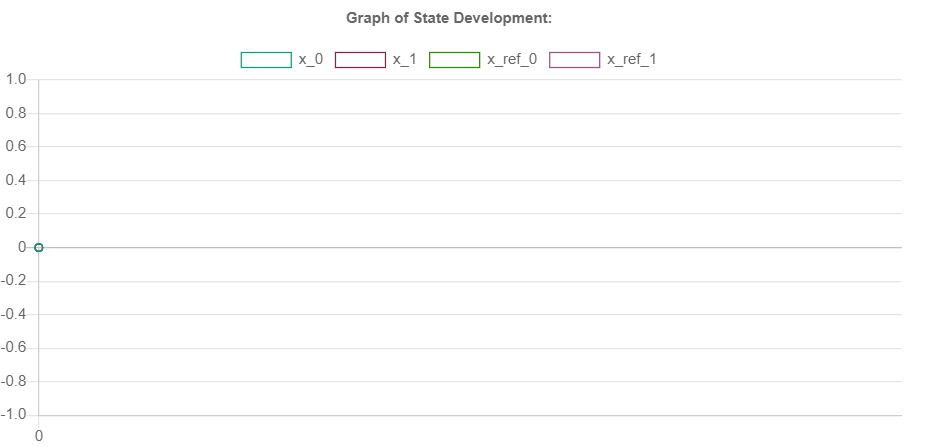
\includegraphics[width=13cm,height=7cm]{images/graf_stavov}
	\caption{Vývoj stavov počas riadenia}
\end{figure}
Na grafe vyššie (Obr. 4.5) bude zobrazený priebeh riadenia jednotlivých stavov a ich referencie.
\begin{figure}[H]	
	\centering
	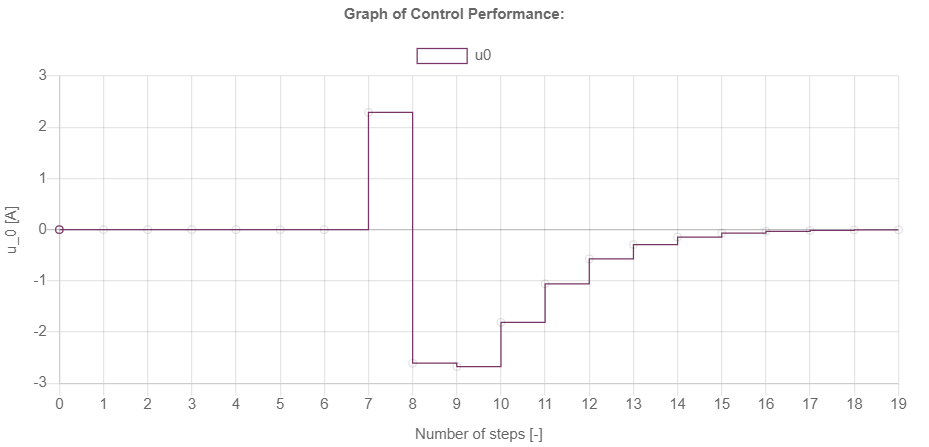
\includegraphics[width=13cm,height=7cm]{images/graf_vstupov}
	\caption{Vývoj akčných zásahov počas riadenia}
\end{figure}
Druhý graf, ktorý budeme mať k dispozícii, je graf vstupov do systému. Bude nám slúžiť pre sledovanie akčných zásahov z MPC.

\section{Logická postupnosť aplikácie}
V tejto podkapitole si rozoberieme rozloženie aplikácie a podrobne si vysvetlíme jej logickú postupnosť. Na \hyperref[fig:ArchitekturaAPK]{(Obr. 4.7)} sme si mohli pozrieť zjednodušený diagram našej aplikácie. Zjednodušený preto, lebo obsahuje iba najhlavnejšie akcie, ktoré sa vykonávajú v aplikácii a je zobrazený iba jeden klient, ktorý otvoril MPC. My si však ideme vysvetliť podrobnejšiu schému, kde si detailne rozoberieme aj menšie akcie a budú v nej zapojení viacerí klienti.
\begin{description}
\item[1. Používateľ 1:]{\hfill
	\begin{enumerate}
		\item{
			Používateľ sa pripojí na http://localhost:5000/, pomocou tlačidla si vyberie prediktívne riadenie (Model Predictive Control), odošle GET request na server. Sever vytvorí nový záznam v \hyperref[DB:Klient]{databáze klientov} a priradí mu vlastné ID. Ako odpoveď mu vráti HTML stránku, kde bude mať na výber vytvoriť nové prediktívne riadenie (New Model Predictive Control), po stlačení bude rovnako presmerovaný na formulár.
		}
		\item{
			Ako sme popísali v časti \hyperref[subse:Formular]{(4.3.1)}, používateľ bude musieť zadefinovať všetky potrebné parametre MPC a všetky potrebné polia pre definovanie modelu systému. Potvrdením sa formulár zvaliduje, ak prejde validáciou je odoslaný na server pomocou request metódy POST.
		}
	\end{enumerate}
}
\item[2. Server:]{\hfill
	\begin{enumerate}
		\item{
			Server spracuje prijaté dáta z formulára, na základe toho či príde diferenciálna rovnica alebo stavový opis systému, upraví tieto rovnice a vytvorí všeobecný model systému. Ostatné dáta sú spracované z textovej podoby do použiteľnej formy.
		}
		\item{
			Následne sú dáta využité pre vytvorenie účelovej funkcie podľa všeobecného vzoru, ktorý sme si ukázali v časti \hyperref[subse:MPC]{(2.1.1)} pre definovaný predikčný horizont $Nmin$. Ak sú zadefinované ohraničenia, tak sa pridajú do účelovej funkcie podľa teórie, ktorú sme si ukázali v časti \hyperref[subse:Ohranicenia]{(2.5.3)}. V ďalšom kroku sa vytvorí nový záznam v \hyperref[DB:OPT]{databáze optimalizačných úloh} so všeobecnými informáciami od používateľa 1.
		}
		\item{
			 Ako posledná úprava sa do účelovej funkcie dosadí vytvorený všeobecný model systému v konkrétnych krokoch predikčného horizontu. Potom sa vytvorí gradient účelovej funkcie vzhľadom k optimalizovaným premenným a vygenerujú sa počiatočné nástrely. Z takýchto údajov sa vytvorí prvý záznam v \hyperref[DB:WORKER]{databáze distribuovaných optimalizačných úloh} a tiež záznam pre každú premennú v \hyperref[DB:WORKER_DATA]{databáze výsledkov po optimalizácií}. Vzhľadom na to, že je prihlásený iba jeden klient, bude sa jednať o normálne centralizované MPC.
		}
		\item{
			Ako odpoveď na prijaté dáta z formulára server vráti HTML stránku spolu s informáciou o IDčku používateľa.
		}
	\end{enumerate}
}
\item[3. Používateľ 1:]{\hfill
\begin{enumerate}
\item{
Používateľ je na poslednej, a zároveň hlavnej HTML stránke, ktorú sme si predstavili v časti \hyperref[subse:OPTaSIM]{(4.3.2)}. Ako prvé sa pripojí cez JavaScript na WebSoket kanál, kde bude odosielať a dostávať správy.
}
\item{
Cez tento komunikačný kanál zašle serveru správu, že je pripravený na prijatie dát. Server mu odpovie zaslaním dát z databáz v podobe Jason
\begin{lstlisting}[language=Python]
{"Klient_ID":[Gradient, Premenna, Hodnota, Funkcia]}
\end{lstlisting}
}
\item{Po obdržaní dát, sa zavolá výpočtový klient (funkcia pre numerickú optimalizáciu) a tá vyrieši optimalizačný problém. Výsledok po optimalizácii sa pošle cez WebSocet kanál na sever a následne sa tento výsledok objaví v \hyperref[fig:Tabulka]{tabuľke výsledkov}.}
\end{enumerate}
}
\item[4. Server:]{\hfill
\begin{enumerate}
\item{
Server dostane dáta a aktualizuje \hyperref[DB:WORKER_DATA]{databázu výsledkov po optimalizácií}. Keďže je stále pripojený iba jeden používateľ, nemáme distribuovanú optimalizačnú úlohu, teda nevyužívame ani ADMM. V takejto situácii považujeme obdržané dáta za optimálne akčné zásahy z MPC.
}
\item{
Server zavolá simuláciu, pomocou vypočítaných akčných zásahov a počiatočných stavov vypočíta nové stavy a aktualizuje ich v \hyperref[DB:WORKER_DATA]{databáze výsledkov po optimalizácií}.
}
\item{
Ako posledný krok vytvorí nové dáta pre optimalizáciu z databázy v podobe Jason a odošle ich cez komunikačný kanál používateľovi.
}
\end{enumerate}
}
\item[5. Používateľ 1:]{\hfill
	\begin{enumerate}
		\item{Klient opäť obdrží dáta, zavolá výpočtového klienta, ten vyrieši optimalizačný problém. Výsledok po optimalizácii sa pošle cez WebSocet kanál na sever a následne sa tento výsledok objaví v \hyperref[fig:Tabulka]{tabuľke výsledkov}.}
	\end{enumerate}
}
\item[6. Cyklus:]{\hfill
	\begin{enumerate}
		\item{V tomto momente vznikne cyklus (od kroku 4. po 5.) a bude sa opakovať, až kým sa nepripojí nový používateľ.}
	\end{enumerate}
}
\item[7. Používateľ 2:]{\hfill
	\begin{enumerate}
		\item{Rovnako ako používateľ 1 sa aj používateľ 2 pripojí k serveru na adrese http://localhost:5000/,  pomocou tlačidla si vyberie prediktívne riadenie. V tomto okamžiku má na výber už z dvoch možností, pripojiť sa k prebiehajúcemu riadeniu (talčidlo Join MPC), alebo môže založiť ďalšie riadenie rovnako ako používateľ 1. Ak by si vybral zloženie nového riadenia, pokračoval by rovnako ako používateľ 1 od kroku 1.}
		\item{
			Po pripojení sa k prebiehajúcemu riadeniu, odošle serveru request a ten mu pošle naspäť HTML stránku a priradí mu ID.
		}
		\item{ 
			Pripojí sa na komunikačný kanál a zašle serveru informáciu o tom, že sa pridal k riadeniu. 
		}
	\end{enumerate}
}
\item[8. Server :]{\hfill
	\begin{enumerate}
		\item{
			Server obdrží správu, že sa pripojil ďalší používateľ k riadeniu a preruší cyklus v korku 6.
		}
		\item{
			Zavolá \hyperref[DB:OPT]{databázu optimalizačných úloh} a nájde príslušné MPC, ku ktorému sa používateľ pripojil. Následne na to si zistí, koľko používateľ je aktívnych a aký je $Nmin$ (minimálny predikčný horizont). Na základe tejto informácie vytvorí decentralizovaný optimalizačný problém zo všeobecnej rovnice a modelu systému. Postupuje podla teórie uvedenej v časti \hyperref[subse:Nelin_MPC_ADMM]{(2.5.2)} s výnimkou, že sa nebude uvažovať plná decentralizácia, ale rozdelí sa počet príslušných korkov predikčného horizontu medzi používateľov.
		}
		\item{
			Po vytvorení distribuovaného optimalizačného problému sa aktualizuje \hyperref[DB:WORKER]{databáza distribuovaných optimalizačných úloh} a \hyperref[DB:WORKER_DATA]{databáza výsledkov po optimalizácii}. S drobnou obmenou sa ako nástrel pre optimalizáciu využijú staré údaje a nebudú sa generovať nové. 
		}
		\item{
			Po aktualizácii údajov server zašle dáta cez komunikačný kanál všetkým používateľom vo formáte Jason.
		}
	\end{enumerate}
}
\item[9. Cyklus:]{\hfill
	\begin{enumerate}
		\item{V tomto momente vznikne nový cyklus, ale komplikovanejší ako bol v kroku 6., pridá sa totiž ADMM k simulácii (budeme mať cyklus v cykle)}
		\item{Používatelia obdržia dáta, zavolajú výpočtových klientov a tí vyriešia optimalizačný problém. Výsledok po optimalizácii sa pošle cez WebSocet kanál na sever a následne sa tento výsledok objaví v \hyperref[fig:Tabulka]{tabuľke výsledkov}.}
		\item{
			Server čaká, kým neobdrží výsledky od všetkých používateľov. Potom spracuje výsledky, aktualizuje databázy a duálnu funkciu. Následne na to vyhodnotí kritériá pre zastavenie ADMM. Ak nie sú splnené, pošle aktualizované dáta používateľom a pokračuje od korku 2 (9. Cyklu). Ak sú kritériá splnené, považujeme výsledok za optimálne akčné zásahy. Ďalej server zavolá simuláciu pomocou vypočítaných akčných zásahov a počiatočných stavov, vypočíta nové stavy a aktualizuje ich v \hyperref[DB:WORKER_DATA]{databáze výsledkov po optimalizácii} a pokračuje od kroku 2 (9. Cyklu).
		}
	\end{enumerate}
}
\end{description}
Vysvetlili sme si princíp fungovania aplikácie pri pripojení dvoch používateľov. Ak by sa pripojilo viac, než dvaja používatelia, nespôsobí to problém, a postup bude vždy rovnaký od korku 7. Zmena môže nastať v dvoch prípadoch.
\begin{enumerate}
	\item{
	 Pripojí sa viac používateľov ako je minimálny predikčný horizont, v takom prípade už máme maximálne decentralizovaný optimalizačný problém. Zmena nastane v tom, že už nemáme k dispozícií žiadny voľní krok predikčného horizontu. Teda je nutné vytvoriť nový krok predikčného horizontu nad rámec minimálneho predikčného horizontu a ten sa priradí používateľovi.
	}
	\item{
	Ak sa nejaký používateľ odpojí z riadenia, preruší sa cyklus v korku 9., na čo server zareaguje ako pri pridaní klienta do riadenia (krok 8.), len miesto toho, aby prepočítal distribúciu optimalizácie o používateľa navyše, odoberie jedného. 
	}
\end{enumerate}
Celú aplikáciu sme zverejnili na githube spolu s možnosťou vytvorenia docker kontajneru link je nasledovný (\url{https://github.com/xkohutr1/Diplomovka.git}). Docker umožňuje spustenie servera na hocikom operačnom systéme a nie je nutné mať nainštalované, žiadne programovacie jazyky alebo špeciálne knižnice.

\section{Experiment}
V poslednej časti tejto kapitoly overíme funkčnosť navrhnutej aplikácie na simulácii, a to pri rovnakých podmienkach, ako v časti \hyperref[sec:HB]{(3.1)}. Prihlásime prvého používateľa, ten zadefinuje všetky potrebné informácie do formulára, ale bez skokovej zmeny, a odošle ho na server. Postupne pridáme štyroch ďalších používateľov, aby sme zabezpečili plnú decentralizáciu optimalizačného problému, ako tomu bolo v časti \hyperref[sec:HB]{(3.1)}. Keď sú všetci používatelia pripravení, vykonáme v kroku $10$ skokovú zmenu pomocou zmeny referencie z počiatočných stavov do nuly.
\begin{center}
	\begin{figure}[H]
		\centering
		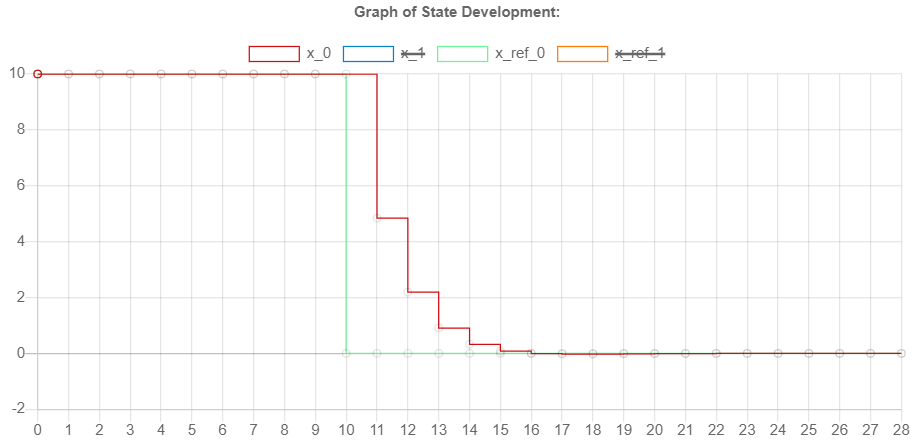
\includegraphics[width=13cm,height=6.5cm]{images/Hmotny_bod_apk/x0}
		\caption{Priebeh riadenia pre prvý stav systému}
	\end{figure}
\end{center}
\begin{figure}[H]
	\centering
	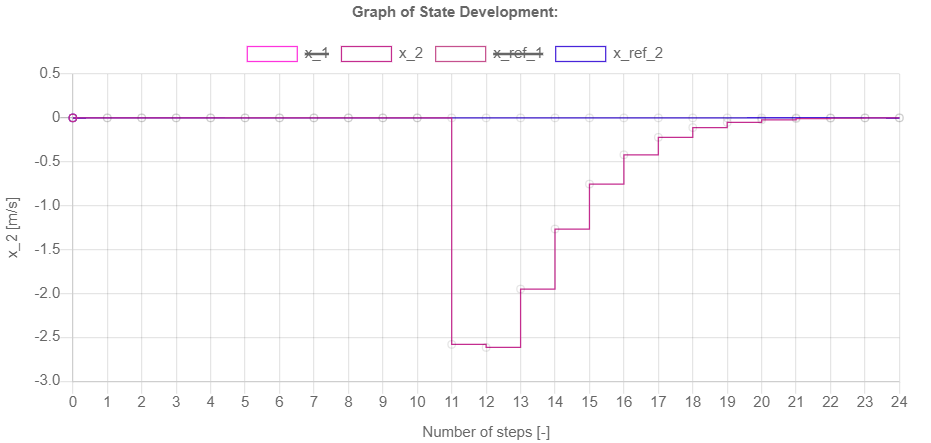
\includegraphics[width=13cm,height=6.5cm]{images/Hmotny_bod_apk/x1}
	\caption{Priebeh riadenia pre druhý stav systému}
\end{figure}
\begin{figure}[H]
	\centering
	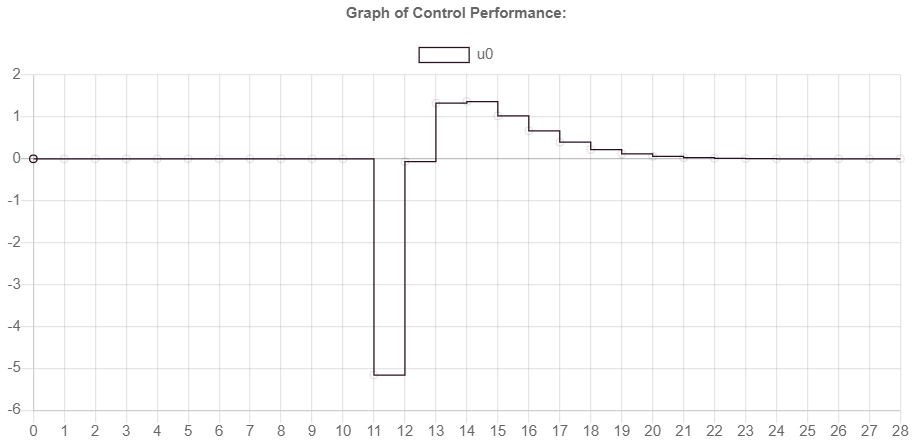
\includegraphics[width=13cm,height=6.5cm]{images/Hmotny_bod_apk/u}
	\caption{Vývoj akčných zásahov}
\end{figure}
Na grafoch (Obr. 4.8 až 4.10) môžeme vidieť priebeh simulácie. Pri porovnaní so simuláciou, ktorú sme vykonali v programovacom jazyku Matlab \hyperref[sec:HB]{(3.1)} zistíme, že sú priebehy totožné, a preto považujeme našu aplikáciu za funkčnú. 